\documentclass{presentation}

\usepackage{tikz}

% some details about the cover page
\title[slide $\text{\insertframenumber}$]{Efficient Algorithm}
\subtitle{Jump points}
\author{Rademacher, Loka}
\date{\today}
\institute{
    Department of Computer Science \\
    University of Bonn
}

\begin{document}


\begin{frame}
    \titlepage
\end{frame}



\begin{frame}{Contents}
    \begin{itemize}
        \item Path finding on grid graphs
        \item A Star Search ($A^\star$)
        \item Jump Point Search ($JPS$)
        \item Jump Point Search Improvements ($JPS^+$)
        \item Bounding Boxes ($BB$)
        \item Defined goal
    \end{itemize}
\end{frame}



\begin{frame}
    \bigbox{Path finding on grid graphs}
\end{frame}

\begin{frame}{Problem definition}
	\begin{minipage}{0.3\textwidth}

	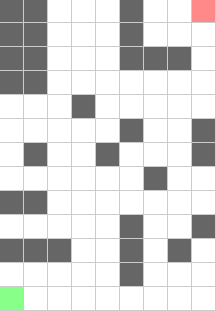
\includegraphics[width=\textwidth]{figures/gridgraph.png}
	
	\end{minipage}%
	\hfill%
	\begin{minipage}{0.6\textwidth}
	

	\begin{itemize}
		\item 4-tuple $(G, s, g, h)$:
		\pause
		\begin{itemize}
		\item[$\tikz{\path[draw=black,fill=white] (0,0) rectangle (2mm,2mm);}$] Euclidean grid graph $G$
		\item[$\tikz{\path[draw=black,fill=white!60!green] (0,0) rectangle (2mm,2mm);}$] start node $s$
		\item[$\tikz{\path[draw=black,fill=white!60!red] (0,0) rectangle (2mm,2mm);}$] goal node $g$
		\item[$\tikz{\path[draw=black,fill=gray] (0,0) rectangle (2mm,2mm);}$] $\not\in G$ obstacle
		\pause
		\item[$\rightarrow$] edge costs $1$
		\item[$\nearrow$] edge costs $\sqrt{2}$
		\pause
		\item[$h$:] a heuristic function
		\end{itemize}
	\end{itemize}
	
	\end{minipage}
	
	\hspace{3cm}
	
	\pause
	\begin{center}
		Goal: shortest path from $s$ to $g$ over $G$
	\end{center}

\end{frame}


\begin{frame}{Heuristic Function $h$}
	\begin{minipage}{0.3\textwidth}
		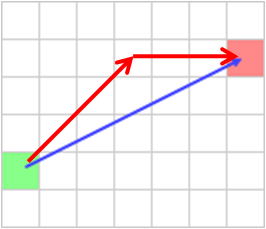
\includegraphics[width=\textwidth]{figures/heuristic.png}
	\end{minipage}%
	\hfill%
	\begin{minipage}{0.6\textwidth}
		\begin{itemize}
		\item $h(\tikz{\path[draw=black,fill=white!60!green] (0,0) rectangle (2mm,2mm);},\tikz{\path[draw=black,fill=white!60!red] (0,0) rectangle (2mm,2mm);})\leq min_{path}(\tikz{\path[draw=black,fill=white!60!green] (0,0) rectangle (2mm,2mm);},\tikz{\path[draw=black,fill=white!60!red] (0,0) rectangle (2mm,2mm);})$
		\pause
		\item e.g.:\\ $h(\tikz{\path[draw=black,fill=white!60!green] (0,0) rectangle (2mm,2mm);},\tikz{\path[draw=black,fill=white!60!red] (0,0) rectangle (2mm,2mm);}) = dist_{euklid}(\tikz{\path[draw=black,fill=white!60!green] (0,0) rectangle (2mm,2mm);},\tikz{\path[draw=black,fill=white!60!red] (0,0) rectangle (2mm,2mm);})$
		\begin{itemize}
			\item $\sqrt{27} \leq 3+3\cdot\sqrt{2}$
		\end{itemize}
		\end{itemize}
	\end{minipage}
\end{frame}


\begin{frame}
    \bigbox{A Star search ($A^\star$)}
\end{frame}


\begin{frame}{Main ideas: Neighborhood}
	\begin{center}
		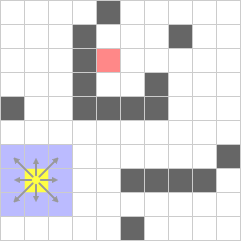
\includegraphics[width=0.5\textwidth]{figures/A-Stern_geschnitten(241x241)/2.png}
	\end{center}
\end{frame}


\begin{frame}{Main ideas: Priority Queue}
Hier muss die Order für die Priority Queue hin. Auf das Bild würde ich dann in die lila felder die zahlen 1-8 reinschreiben, der Order nach. Man könnte zusätzlich noch Pfeile wie bei der Heuristic zeichnung reinmachen, ganz wie du das magst (immerhin sollst du den teil ja vortragen)
Hier passen die Bilder irgendwie weder zu "weg bisher+euklid", noch zu "nimm den kürzesten weg bis her und bei gleichstand euklid". Beides würde sinn ergeben, sind aber wiedersprüche zu den bildern =( Bei JPS klappt es mit addition
	\begin{center}
		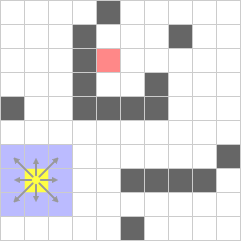
\includegraphics[width=0.5\textwidth]{figures/A-Stern_geschnitten(241x241)/2.png}
	\end{center}
\end{frame}


\begin{frame}{Example}
	\begin{minipage}{0.2\textwidth}
		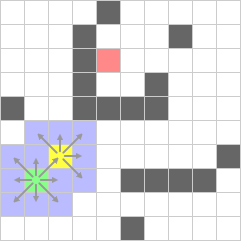
\includegraphics[width=\textwidth]{figures/A-Stern_geschnitten(241x241)/3.png}
	\end{minipage}%
	\hfill%
	\begin{minipage}{0.2\textwidth}
		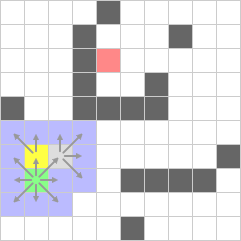
\includegraphics[width=\textwidth]{figures/A-Stern_geschnitten(241x241)/4.png}
	\end{minipage}%
	\hfill%
	\begin{minipage}{0.2\textwidth}
		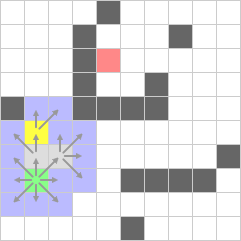
\includegraphics[width=\textwidth]{figures/A-Stern_geschnitten(241x241)/5.png}
	\end{minipage}%
	\hspace{3cm}
	\begin{minipage}{0.2\textwidth}
		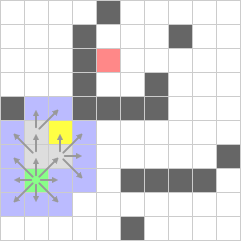
\includegraphics[width=\textwidth]{figures/A-Stern_geschnitten(241x241)/6.png}
	\end{minipage}%
	\hfill%
	\begin{minipage}{0.2\textwidth}
		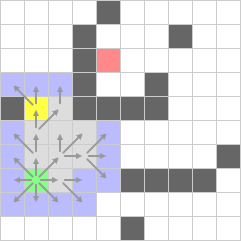
\includegraphics[width=\textwidth]{figures/A-Stern_geschnitten(241x241)/7.png}
	\end{minipage}%
	\hfill%
	\begin{minipage}{0.2\textwidth}
		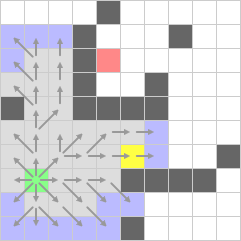
\includegraphics[width=\textwidth]{figures/A-Stern_geschnitten(241x241)/8.png}
	\end{minipage}%
	\hspace{3cm}
	\begin{minipage}{0.2\textwidth}
		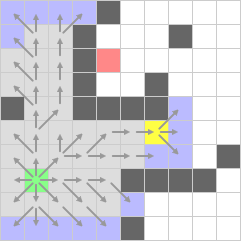
\includegraphics[width=\textwidth]{figures/A-Stern_geschnitten(241x241)/9.png}
	\end{minipage}%
	\hfill%
	\begin{minipage}{0.2\textwidth}
		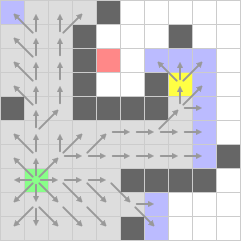
\includegraphics[width=\textwidth]{figures/A-Stern_geschnitten(241x241)/10.png}
	\end{minipage}%
	\hfill%
	\begin{minipage}{0.2\textwidth}
		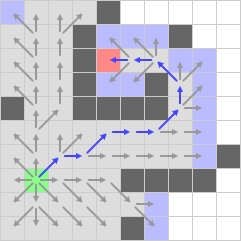
\includegraphics[width=\textwidth]{figures/A-Stern_geschnitten(241x241)/11.png}
	\end{minipage}%	
\end{frame}


\begin{frame}{Symmetric paths}
	\begin{center}
		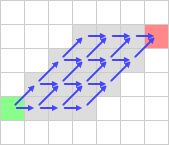
\includegraphics[width=0.5\textwidth]{figures/symmetricpath.png}
	\end{center}
\end{frame}

\begin{frame}
    \bigbox{Jump Point Search ($JPS$)}
\end{frame}



\begin{frame}
    \bigbox{Jump Point Search Improvements ($JPS^+$)}
\end{frame}



\begin{frame}
    \bigbox{Bounding Boxes ($BB$)}
\end{frame}



\begin{frame}
    \bigbox{Defined goal}
\end{frame}



\begin{frame}
    \bigbox{Thanks for attention!}
\end{frame}


\end{document}
